% ============================================================================
% MÓDULO 1 - FUNDAMENTOS EPISTEMOLÓGICOS E CONCEITUAIS DA ANÁLISE AMBIENTAL
% CAPÍTULO 2 - A MODERNIDADE, A GEOGRAFIA E A RELAÇÃO SOCIEDADE-NATUREZA
% ============================================================================

\chapter{A Modernidade, a Geografia e a Relação Sociedade-Natureza}
\noindent\tagEmenta\ \tagEO{1}\par\vspace{6pt}

% ----------------------------------------------------------------------------
% ETAPA 1 - OBJETIVOS DE APRENDIZAGEM
% ----------------------------------------------------------------------------
\begin{capObjetivos}
Ao concluir este capítulo, base direta para a elaboração do \textbf{Estudo Orientado 1 (EO1)}, você será capaz de:
\begin{enumerate}[leftmargin=1.6em, itemsep=2.5pt]
  \item Compreender a formação histórica da questão ambiental na modernidade e o papel da ruptura cartesiana na separação entre sociedade e natureza.
  \item Analisar a tese de Carlos Walter Porto-Gonçalves (2006, p. 8--36) de que a natureza é também uma construção social e historicamente instituída por cada cultura.
  \item Explicar como a racionalidade instrumental converte elementos naturais em ``recursos'' e mercadorias, gerando descompasso entre o tempo econômico e os tempos ecológicos.
  \item Interpretar conflitos socioambientais como disputas pela produção do espaço geográfico, analisando frentes concretas da Bahia e do Nordeste (expansão energética, barragens, fronteira agrícola e acesso à água).
  \item Introduzir os fundamentos da abordagem socioambiental proposta por Francisco Mendonça (2001) para superar a dicotomia clássica entre Geografia Física e Geografia Humana.
\end{enumerate}
\end{capObjetivos}

% ----------------------------------------------------------------------------
% ETAPA 2 - REVISÃO DE PRÉ-REQUISITOS
% ----------------------------------------------------------------------------
\begin{capRevisao}
Este capítulo aprofunda diretamente os debates abertos na Semana 1. Antes de iniciar a leitura, assegure-se de recordar:
\begin{itemize}[leftmargin=1.5em, itemsep=2.5pt]
  \item \textbf{Crise de racionalidade (Cap. 1),} a crise ambiental contemporânea resulta da racionalidade econômica dominante e da fragmentação do conhecimento (Leff, 2001).
  \item \textbf{Crítica ao desenvolvimento sustentável (Cap. 1),} o modo como nomeamos e conceituamos o ambiente envolve disputas políticas e projetos distintos de sociedade (Porto-Gonçalves, 2006).
  \item \textbf{Dualismo na história da Geografia,} desde sua institucionalização acadêmica no século XIX, a Geografia conviveu com a tensão entre abordagens voltadas aos fenômenos físico-naturais e abordagens centradas nas dinâmicas socioeconômicas e culturais.
\end{itemize}
\end{capRevisao}

% ----------------------------------------------------------------------------
% ETAPA 3 - EXPLICAÇÃO TEÓRICA
% ----------------------------------------------------------------------------
\etapa{3}{Fundamentação Teórica: Modernidade, Apropriação da Natureza e Conflitos Territoriais}

\begin{boxSimbolo}[Vocabulário Técnico e Conceitos-Chave do Capítulo]
Na análise histórica da questão ambiental, a \textbf{Modernidade} designa o projeto filosófico, científico e econômico consolidado entre os séculos XVI e XVIII em torno do progresso linear, da ciência mecanicista e do domínio técnico da natureza. Seu núcleo epistemológico reside na \textbf{ruptura cartesiana} entre sujeito pensante (\emph{res cogitans}) e matéria externa (\emph{res extensa}), que legitimou a \textbf{racionalidade instrumental} voltada ao cálculo de meios eficientes de controle e retorno econômico. Nesse percurso, Porto-Gonçalves (2006) mostra que a \textbf{natureza como construção social} convive com sua materialidade física, enquanto um \textbf{recurso natural} só adquire essa condição mediante \textbf{apropriação da natureza} por um sistema técnico e jurídico específico. Disputas assimétricas na \textbf{produção do espaço} originam \textbf{conflitos socioambientais}, cujo exame integrado fundamenta a \textbf{abordagem socioambiental} de Mendonça (2001).
\end{boxSimbolo}

\section{Formação Histórica da Questão Ambiental na Modernidade}

A forma como hoje falamos em ``meio ambiente'', ``recursos naturais'' ou ``impacto ambiental'' resulta de uma longa transformação histórica iniciada na transição da Idade Média para a \textbf{Modernidade} europeia, intensificada pela expansão marítimo-colonial a partir do final do século XV, pela Revolução Científica dos séculos XVI e XVII e pela Revolução Industrial a partir do século XVIII. Durante esse processo, alterou-se profundamente tanto a base material da produção quanto a visão de mundo que legitimava a intervenção humana sobre o planeta. A expansão colonial incorporou vastos territórios das Américas, da África e da Ásia às rotas comerciais europeias, reorganizando ecossistemas inteiros em torno de produtos primários como açúcar, metais preciosos, madeira, algodão e café. Na etapa industrial, o uso massivo de combustíveis fósseis (inicialmente carvão mineral e, depois, petróleo) rompeu a dependência exclusiva da força muscular, animal e hidráulica local, multiplicando em escala sem precedentes a capacidade humana de alterar relevos, cursos d'água, solos e atmosfera.

\subsection{A Ruptura Cartesiana entre Sociedade e Natureza}

Essa transformação material foi acompanhada e filosoficamente legitimada por uma mudança radical no modo de pensar. Filósofos e cientistas fundadores da ciência moderna, como Francis Bacon e René Descartes, consolidaram uma concepção mecanicista do mundo. Na formulação cartesiana, estabeleceu-se uma cisão ontológica entre o sujeito racional humano (\emph{res cogitans}) e a matéria extensa (\emph{res extensa}), isto é, a natureza externa. A natureza passou a ser comparada a uma grande máquina regida por leis matemáticas decifráveis, de modo que conhecê-la passou a significar \textbf{dominá-la, controlá-la e submetê-la} aos desígnios humanos.

Essa \textbf{ruptura moderna entre sociedade e natureza} produziu consequências decisivas para a Análise Ambiental ao externalizar o mundo natural, fragmentar o saber científico e cindir a própria Geografia (Figura~\ref{fig:sociedade-natureza}). Por meio da \textbf{externalização da natureza}, o ser humano passou a conceber-se fora e acima do mundo natural, tratando rios, florestas e solos como objetos externos disponíveis à exploração contínua. Essa postura epistemológica alimentou a \textbf{fragmentação científica}, dividindo o conhecimento entre as ciências da natureza (dedicadas ao mundo físico-biológico) e as ciências humanas (voltadas à cultura e à economia). Ao institucionalizar-se como ciência moderna no século XIX, a própria Geografia absorveu essa fratura e estruturou uma \textbf{dicotomia interna} entre uma Geografia Física orientada às leis naturais e uma Geografia Humana focada na sociedade, superada contemporaneamente pela abordagem socioambiental.

\begin{figure}[H]
  \centering
  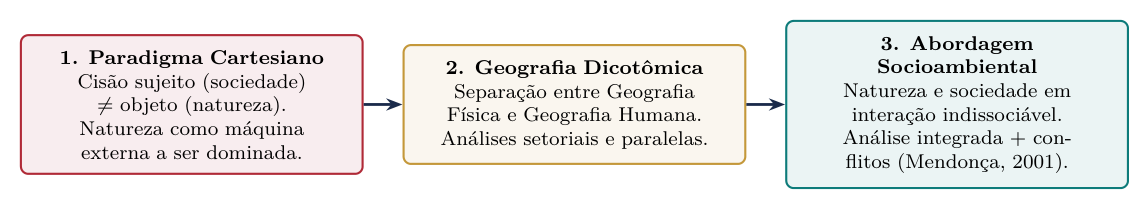
\includegraphics[width=0.92\textwidth]{figures/esquema_sociedade_natureza.png}
  \caption{Percurso histórico-epistemológico da ruptura cartesiana e da Geografia dicotômica até a emergência da abordagem socioambiental integrada (elaborado com base em Mendonça, 2001).}
  \label{fig:sociedade-natureza}
\end{figure}

\section{A Natureza como Construção Social e Histórica (Porto-Gonçalves, 2006)}

Nas páginas 8 a 36 de \emph{Os (des)caminhos do meio ambiente} (2006), Carlos Walter Porto-Gonçalves desenvolve uma tese central para a formação em Geografia, afirmando que \textbf{toda sociedade e toda cultura cria, inventa e institui uma determinada ideia do que seja a natureza}. Essa afirmação merece atenção rigorosa para evitar leituras simplistas. Reconhecer que a natureza é uma \emph{construção social e histórica} afirma a existência material objetiva da chuva, das rochas, da gravidade e dos processos biológicos, ao mesmo tempo em que destaca que o modo como os seres humanos percebem, classificam, valorizam e se relacionam com esses elementos varia profundamente ao longo da história e entre diferentes culturas.

Ao longo do tempo, diferentes matrizes histórico-culturais instituíram concepções distintas de natureza com expressões espaciais próprias (Porto-Gonçalves, 2006, p. 8--36). Em visões pré-modernas e entre povos indígenas e comunidades tradicionais brasileiras, rios, serras e matas constituem uma totalidade viva e um território de memória, pertencimento e reprodução comunitária, orientando manejos adaptados aos ciclos sazonais, como as áreas de uso comum no Semiárido (Figura~\ref{fig:potigua_cap2}).

\begin{figure}[H]
  \centering
  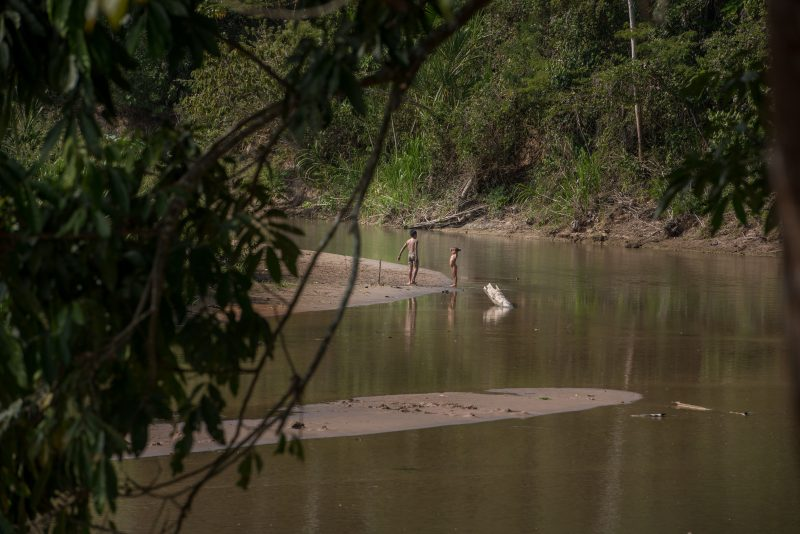
\includegraphics[width=0.76\textwidth]{figures/potigua.jpg}
  \caption{Território indígena e tradicional, expressando a natureza como espaço de vida, memória e pertencimento coletivo. Fonte: Acervo didático CHF662.}
  \label{fig:potigua_cap2}
\end{figure}

Em contraste histórico com essa territorialidade, a modernidade cartesiana e industrial concebeu a natureza como máquina externa e estoque mensurável de recursos sob dominação técnica contínua, multiplicando grandes obras, monoculturas, urbanização acelerada e frentes extrativas de alto impacto como a mineração industrial em larga escala (Figura~\ref{fig:grandes_minas_cap2}). Porto-Gonçalves (2006) aponta ainda um paradoxo revelador da modernidade, pois, paralelamente à devastação urbano-industrial, consolidou-se um preservacionismo excludente que romantiza a ``natureza intocada'' pela ausência humana e cria ilhas de proteção em conflito com moradores locais. Tanto o produtivismo quanto o preservacionismo excludente compartilham a raiz cartesiana que opõe sociedade e natureza como polos excludentes, fratura superada apenas pela perspectiva socioambiental crítica que articula materialidade biofísica, cultura, justiça territorial e convivência regional.

\begin{figure}[H]
  \centering
  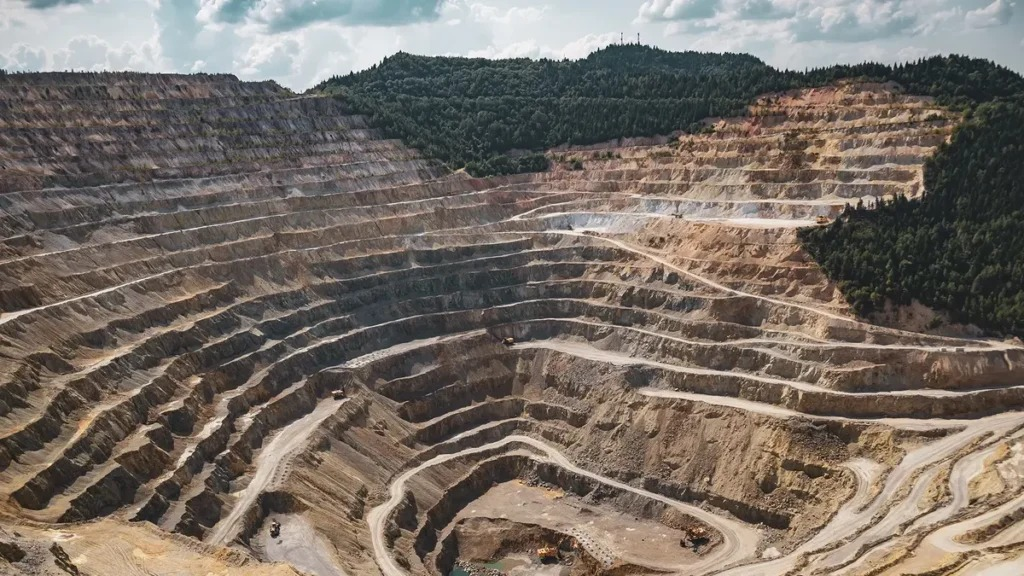
\includegraphics[width=0.76\textwidth]{figures/grandes_minas.jpg}
  \caption{Mineração industrial em larga escala, exemplificando a redução do relevo e do subsolo a mercadoria e estoque extrativo sob a racionalidade instrumental. Fonte: Acervo didático CHF662.}
  \label{fig:grandes_minas_cap2}
\end{figure}

O Exemplo 2.1 mostra como a concepção de ``natureza intocada'' reaparece em relatórios ambientais contemporâneos, reproduzindo o dualismo cartesiano.

\begin{boxExemplo}{2.1 (Básico)}{Identificando o Dualismo Cartesiano em um Relatório Ambiental}
\passoEnunciado{Para criar uma unidade de conservação de proteção integral em uma serra fictícia da Bahia \textit{(cenário didático ilustrativo)}, uma consultoria entregou um relatório técnico dividido em duas partes sem conexão. O Volume 1 descreve a flora e as nascentes como ``patrimônio natural puro'', e o Volume 2 recomenda a retirada imediata de 35 famílias que vivem há três gerações na área praticando extrativismo de baixa intensidade e manejo comunitário de pastagens, classificando qualquer presença humana como ``fator de destruição da natureza''.}
\passoDados{Relatório dividido em dois volumes isolados; idealização da área como ``natureza pura''; recomendação de remoção de 35 famílias tradicionais sem avaliar seus modos históricos de manejo.}
\passoPedido{Identificar qual concepção de natureza fundamenta o relatório à luz de Porto-Gonçalves (2006) e explicar por que essa postura reproduz o dualismo moderno.}
\passoMetodo{Análise epistemológica das concepções de natureza e do paradoxo preservacionista excludente em Porto-Gonçalves (2006, p. 8--36).}
\passoContas{%
\textbf{Passo 1, Concepção subjacente.} O relatório adota o mito da ``natureza intocada'', definindo o natural exclusivamente pela ausência de seres humanos.\\
\textbf{Passo 2, Raiz cartesiana (Porto-Gonçalves, 2006).} Embora aparente opor-se à exploração predatória, essa visão parte da mesma ruptura moderna que separa rigidamente sociedade e natureza em polos excludentes.\\
\textbf{Passo 3, Equívoco geográfico e social.} Ao tratar todas as formas de presença humana como igualmente destrutivas, a consultoria ignora que os modos de manejo tradicional dessas 35 famílias podem ter contribuído para conservar a cobertura vegetal e as nascentes ao longo de gerações, gerando um conflito socioambiental desnecessário.}
\passoResposta{O relatório fundamenta-se na concepção dicotômica da ``natureza intocada'', herdeira da ruptura cartesiana entre sociedade e natureza, ao opor automaticamente conservação ambiental e presença de populações tradicionais.}
\passoVerificacao{A crítica é coerente com a Análise Ambiental contemporânea, pois conservar nascentes exige avaliar empiricamente o impacto real de cada prática de uso da terra, diferenciando manejo comunitário de baixo impacto de pressões predatórias externas.}
\end{boxExemplo}

Ao estudar a tese de Porto-Gonçalves (2006), um equívoco recorrente consiste em interpretar a ideia de construção social como negação da realidade material dos processos naturais, conforme destacado no alerta a seguir.

\begin{boxErro}[Erro 2.1: Confundir ``Natureza como Construção Social'' com Negação da Materialidade Física]
\textbf{Equívoco frequente:} interpretar a tese de Porto-Gonçalves (2006) como se a erosão, as chuvas ou os processos geológicos fossem apenas ``invenções da mente humana'' sem realidade material.

\textbf{Por que está incorreto:} a materialidade biofísica existe objetivamente e obedece a leis físicas, químicas e biológicas. O que é social e historicamente construído é a \emph{ideia} de natureza, o significado cultural que lhe atribuímos e as formas técnicas e econômicas pelas quais a apropriamos e transformamos.

\textbf{Como evitar:} afirme sempre a dupla dimensão segundo a qual os processos naturais possuem dinâmica material própria, enquanto sua apropriação, valoração e interpretação são mediadas pela história e pela sociedade.
\end{boxErro}

\section{Apropriação dos Recursos Naturais e Racionalidade Instrumental}

Sob a modernidade capitalista, os elementos biofísicos da superfície terrestre passam por um processo sistemático de conversão em \textbf{recursos naturais}. Esse detalhe conceitual mostra-se decisivo na Geografia, pois a água, o vento, o solo ou um mineral existem independentemente da economia, adquirindo a condição de ``recursos'' quando um grupo social dispõe de técnica, demanda econômica e respaldo jurídico-político para se apropriar deles. Ao redigir diagnósticos ambientais, o(a) geógrafo(a) distingue três níveis operacionais interligados, começando pelo \textbf{elemento natural} em sua dinâmica biofísica (como o regime de ventos nas serras do Semiárido ou a água infiltrada em um aquífero), passando ao \textbf{recurso natural} quando incorporado por técnicas e finalidades sociais específicas (como o potencial eólico mapeado para geração elétrica ou a água captada para irrigação) e alcançando a condição de \textbf{mercadoria} quando esse recurso é apropriado privadamente e submetido à lógica de compra, venda e especulação. Grande parte dos conflitos socioambientais nasce quando um bem essencial à reprodução comunitária é transformado em mercadoria excludente.

Assim, a \textbf{apropriação dos recursos naturais} é guiada por uma \textbf{racionalidade instrumental} na qual a técnica é mobilizada para acelerar o giro do capital, ampliar a escala de extração e reduzir custos privados de produção. Disso decorre um descompasso estrutural entre duas temporalidades que governam o espaço geográfico (Figura~\ref{fig:temporalidades}). De um lado, o \textbf{tempo do capital}, rápido e linear, exige retorno financeiro em poucos anos, colheitas sucessivas, ampliação acelerada de redes energéticas e expansão contínua sobre novas fronteiras de terra e água. De outro lado, o \textbf{tempo da natureza}, lento e cíclico, envolve décadas para a regeneração florestal da Caatinga e do Cerrado, séculos para a formação de centímetros de solo fértil e ciclos plurianuais para a recarga de aquíferos subterrâneos.

\begin{figure}[H]
  \centering
  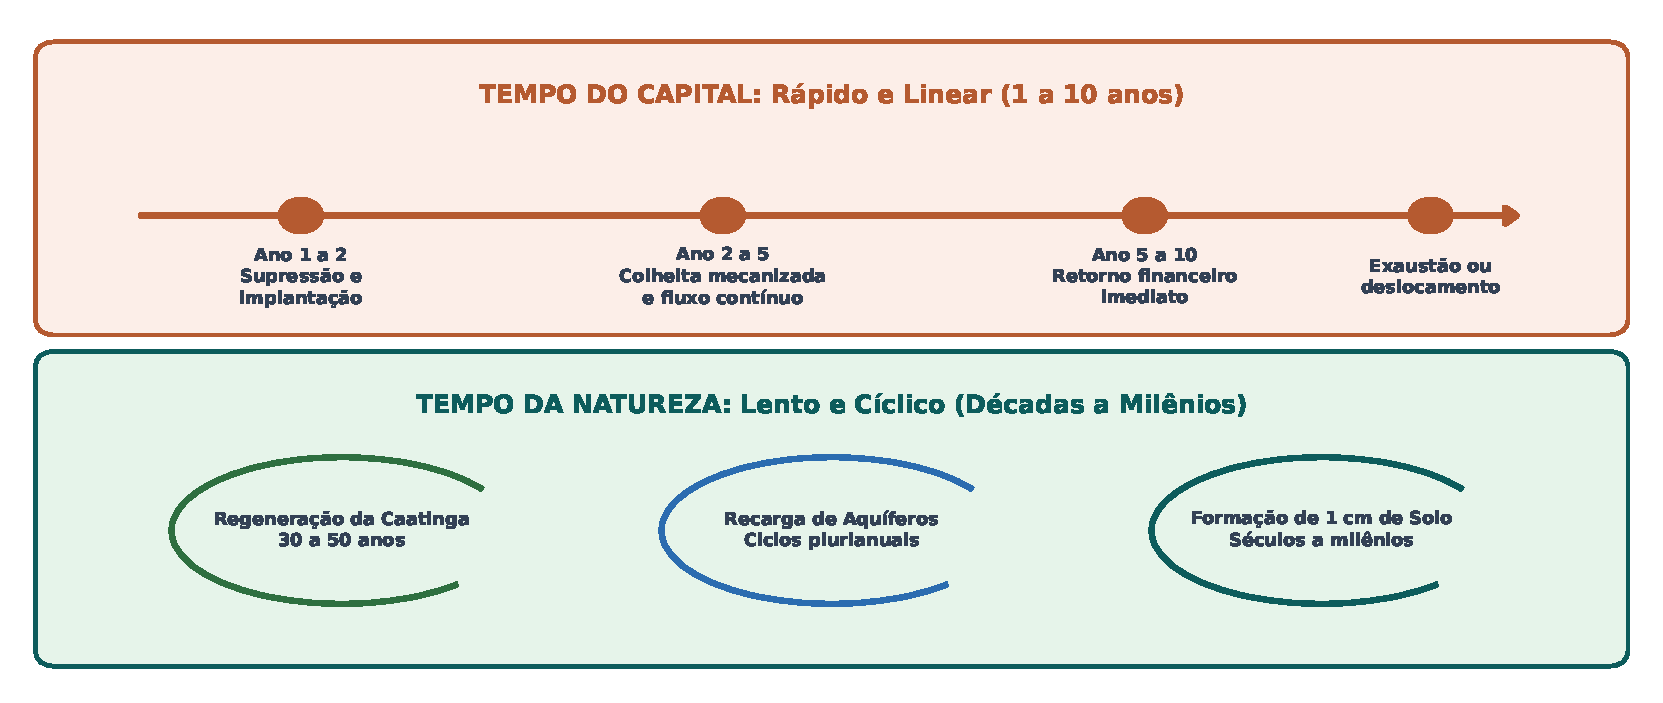
\includegraphics[width=0.94\textwidth]{figures/fig_cap02_temporalidades.pdf}
  \caption{Descompasso de temporalidades entre o tempo linear do capital (retorno em 1 a 10 anos) e o tempo cíclico da natureza (regeneração da Caatinga, recarga de aquíferos e pedogênese em décadas a milênios). Fonte: Elaboração didática CHF662 com base em Leff (2001) e Porto-Gonçalves (2006).}
  \label{fig:temporalidades}
\end{figure}

O Exemplo 2.2 ilustra como um elemento biofísico permanente no sertão baiano adquire o estatuto de recurso econômico e reconfigura relações fundiárias e ambientais.

\begin{boxExemplo}{2.2 (Básico)}{Da Natureza ao Recurso Natural: o Vento nas Serras do Semiárido}
\passoEnunciado{Durante décadas, os ventos intensos que sopram no topo de uma serra da Caatinga \textit{(cenário didático ilustrativo)} eram percebidos pelos moradores locais apenas como parte do clima cotidiano, influenciando a secagem do solo e o manejo dos rebanhos em áreas de uso comum. Nos últimos cinco anos, após o avanço de turbinas de grande porte, o mapeamento anemométrico e a instalação de uma subestação elétrica próxima, o mesmo vento passou a atrair grandes investimentos e contratos de arrendamento de terras para implantação de um complexo eólico.}
\passoDados{Elemento biofísico preexistente dado pelo regime de ventos intensos na serra; novos fatores históricos e técnicos envolvendo aerogeradores de grande porte, mapeamento de potencial eólico e proximidade de linhas de transmissão; consequência marcada por revalorização fundiária e contratos de arrendamento.}
\passoPedido{Explicar, com base na distinção entre \emph{elemento natural} e \emph{recurso natural}, por que o vento adquiriu valor econômico territorial apenas recentemente e quais tensões socioambientais podem emergir.}
\passoMetodo{Análise geográfica do processo de apropriação dos recursos naturais e da produção do espaço sob racionalidade instrumental.}
\passoContas{%
\textbf{Passo 1, De elemento natural a recurso.} O vento sempre existiu fisicamente na serra, mas só se converteu em \emph{recurso energético} quando condições técnicas (aerogeradores), infraestruturais (linhas de transmissão) e econômicas (mercado de energia) permitiram sua apropriação rentável.\\
\textbf{Passo 2, Reconfiguração espacial.} A implantação das torres exige estradas de acesso largas, bases de concreto e faixas de servidão, o que altera a cobertura de Caatinga, expõe o solo à erosão na base das torres e interfere na avifauna.\\
\textbf{Passo 3, Tensões socioambientais emergentes.} O cercamento de áreas antes usadas coletivamente, a assimetria na negociação de contratos de arrendamento e o desconforto acústico próximo às moradias transformam um projeto de ``energia renovável'' em arena de conflito territorial quando falta planejamento socioambiental justo.}
\passoResposta{O vento tornou-se recurso natural apenas quando incorporado por um conjunto técnico, infraestrutural e econômico específico; sua apropriação reorganiza o território da serra e pode gerar impactos físicos e conflitos fundiários com comunidades locais.}
\passoVerificacao{O exemplo antecipa uma lição-chave para a viagem de campo da Semana 11 (eixo de Canudos), mostrando que ser fonte renovável mantém a necessidade de avaliar impactos ambientais e conflitos territoriais.}
\end{boxExemplo}

\section{Conflitos Socioambientais e Produção do Espaço na Bahia e no Nordeste}

A apropriação desigual dos recursos naturais nunca ocorre em um espaço vazio. Todo território já é ocupado, manejado e significado por diferentes grupos sociais (comunidades camponesas, quilombolas, indígenas, pescadores artesanais, agricultores familiares, moradores urbanos, empresas e Estado). Quando um empreendimento ou política altera a qualidade do solo, o regime das águas, o acesso à terra ou o modo de vida local em benefício de determinados agentes e em prejuízo de outros, emergem \textbf{conflitos socioambientais}. Um conflito socioambiental constitui uma disputa concreta pela \textbf{produção do espaço geográfico}, na qual diferentes atores defendem usos incompatíveis ou assimétricos para o mesmo território. No Nordeste brasileiro e no estado da Bahia, quatro frentes territoriais exemplificam essa dinâmica.

Na frente de \textbf{expansão energética} no Semiárido Baiano, a combinação entre ventos constantes nas serras e chapadas, topografia favorável e proximidade de linhas de transmissão transformou áreas de Caatinga e espaços de uso rural em polos eólicos e solares (tema direto da Viagem de Campo da Semana~11). Embora apresentadas como fontes limpas de carbono, essas instalações modificam a paisagem imediata das comunidades rurais ao inserir aerogeradores de grande porte junto a moradias e cercados familiares (Figura~\ref{fig:parque_eolico_rural}), além de envolver supressão vegetal para plataformas e parques fotovoltaicos extensivos (Figura~\ref{fig:solar_desmatamento}), abertura de acessos pesados, compactação e erosão na base das torres, ruído contínuo e contratos assimétricos de arrendamento com famílias de fundo de pasto.

\begin{figure}[H]
  \centering
  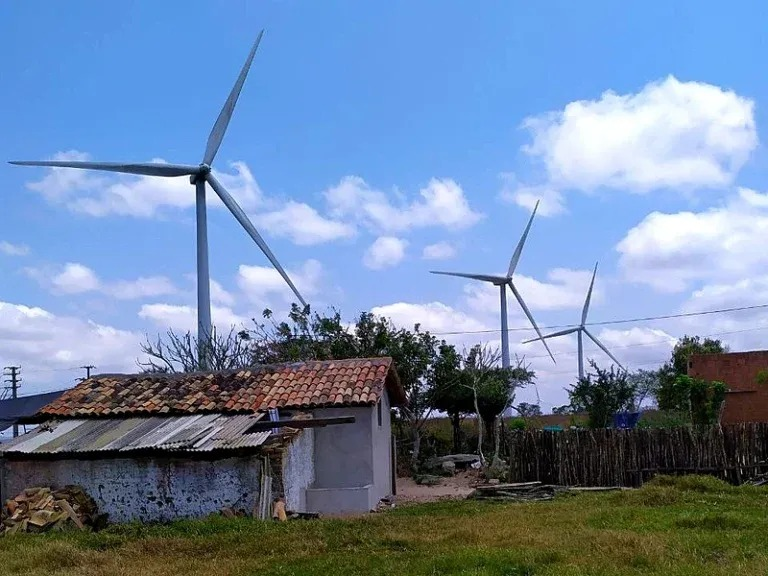
\includegraphics[width=0.76\textwidth]{figures/foto_parque_eolico_rural.jpg}
  \caption{Aerogeradores instalados em proximidade direta a moradias rurais no Semiárido, ilustrando a convivência cotidiana entre infraestruturas energéticas, ruído e organização espacial camponesa. Fonte: Acervo didático CHF662.}
  \label{fig:parque_eolico_rural}
\end{figure}

\begin{figure}[H]
  \centering
  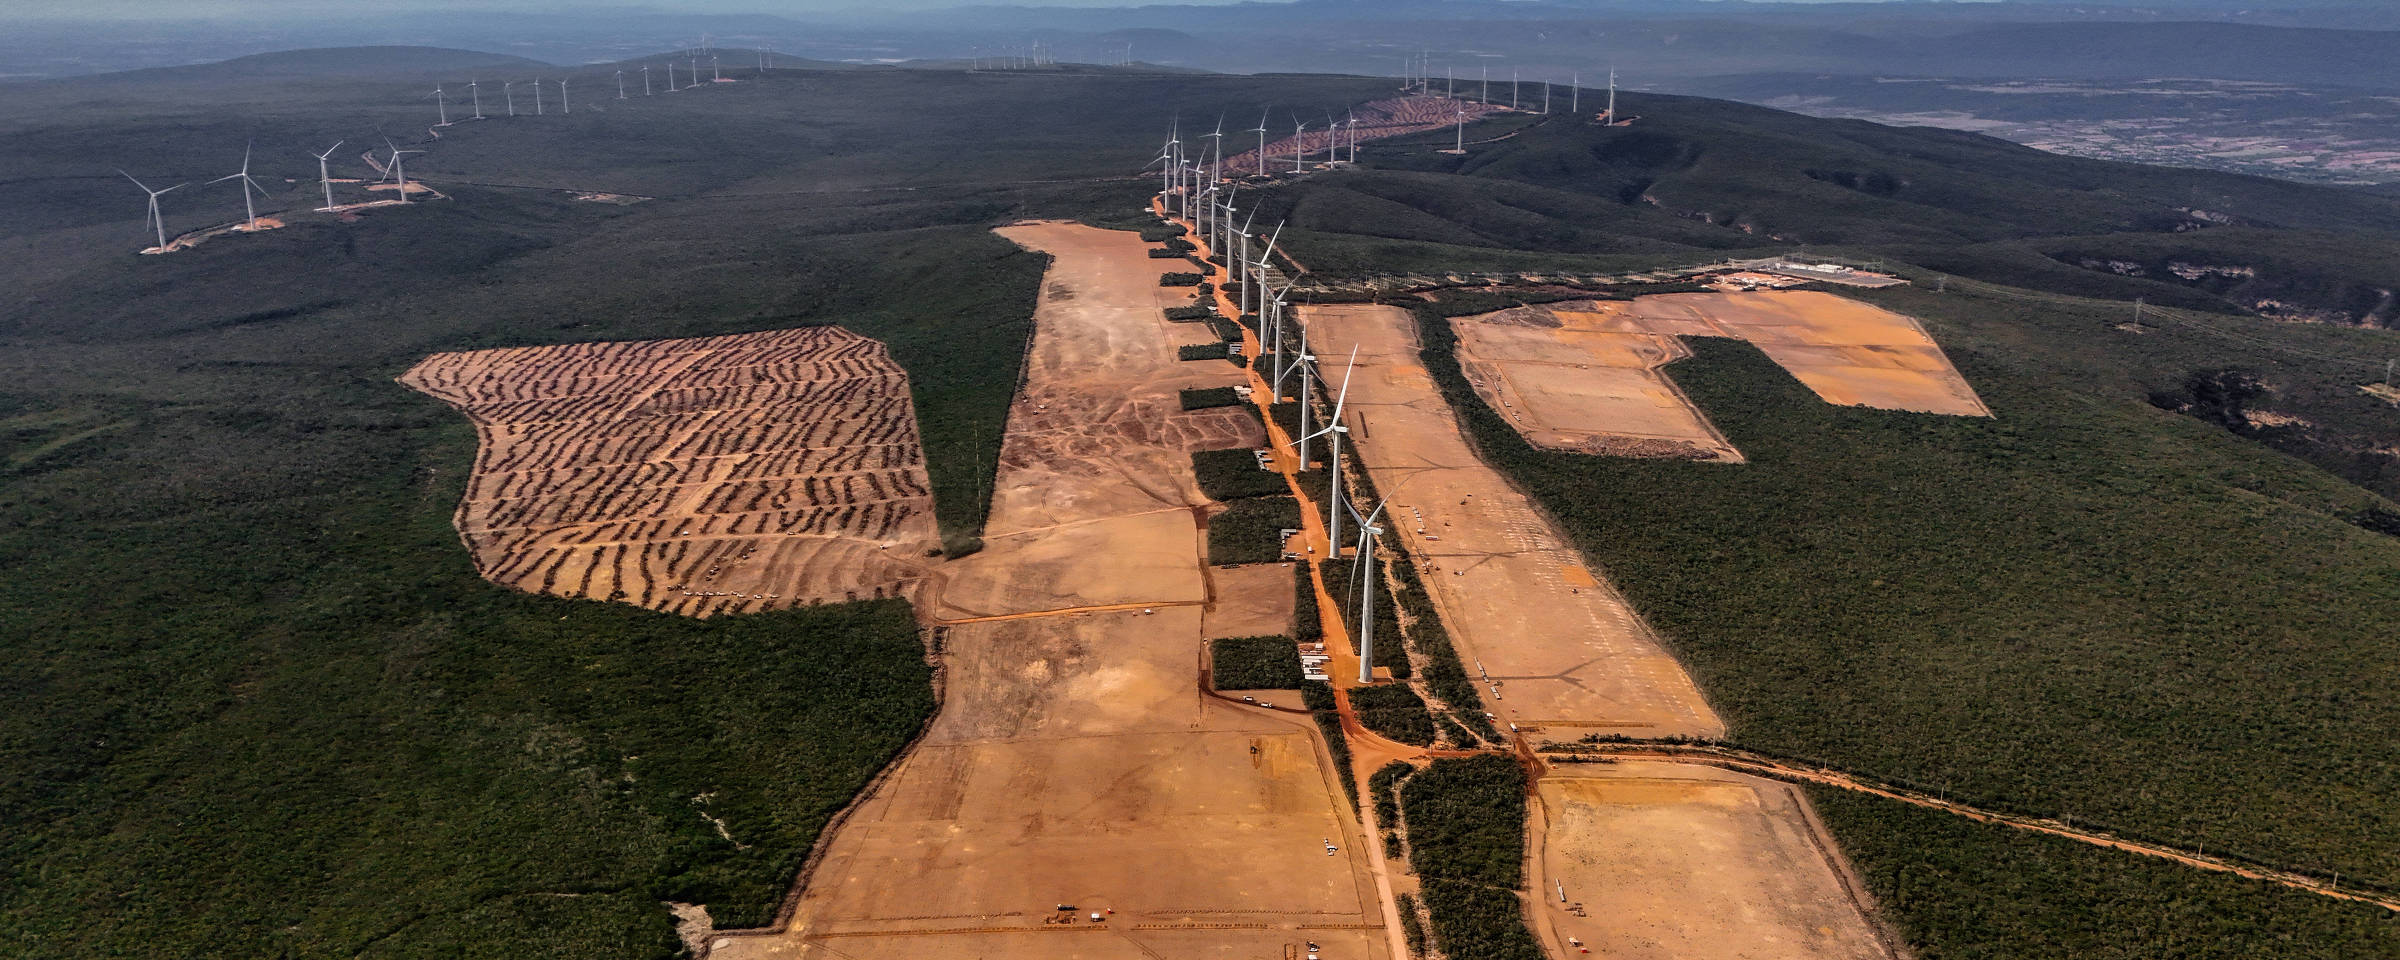
\includegraphics[width=0.76\textwidth]{figures/solar_desmatamento.jpg}
  \caption{Supressão da vegetação nativa associada à implantação de infraestrutura energética no Semiárido, evidenciando alterações na cobertura superficial e na dinâmica erosiva. Fonte: Acervo didático CHF662.}
  \label{fig:solar_desmatamento}
\end{figure}

Na frente das \textbf{barragens e grandes empreendimentos hídricos}, a construção de reservatórios de grande porte e projetos de regularização fluvial no Nordeste e na bacia do rio São Francisco, como a UHE Sobradinho (Figura~\ref{fig:sobradinho_barragem}), reconfigurou profundamente vales inteiros. Ao lado da geração hidrelétrica e da oferta de água para polos irrigados, esses empreendimentos implicaram o alagamento de terras férteis de vazante, o deslocamento compulsório de populações ribeirinhas, a alteração do pulso natural de cheias e vazantes e mudanças na dinâmica hidrossedimentológica a jusante, afetando a pesca artesanal e acelerando a erosão marginal.

\begin{figure}[H]
  \centering
  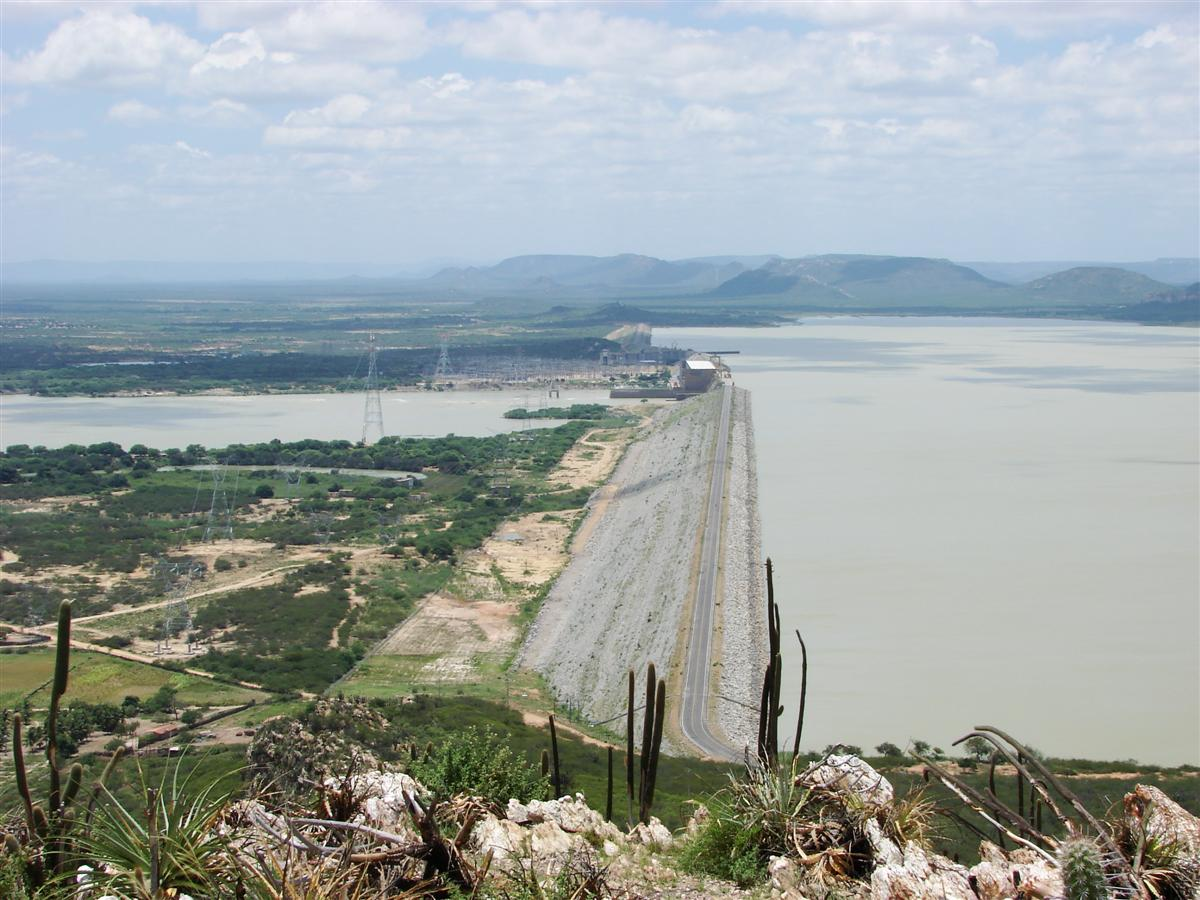
\includegraphics[width=0.76\textwidth]{figures/Barragem_de_Sobradinho-BA.jpg}
  \caption{Barragem da Usina Hidrelétrica de Sobradinho no Rio São Francisco (BA), marco da regularização de vazões e da reorganização territorial do vale. Fonte: Acervo didático CHF662.}
  \label{fig:sobradinho_barragem}
\end{figure}

Para compreender quantitativamente como disputas pela água em reservatórios expressam apropriação desigual, o Exemplo 2.3 analisa um balanço volumétrico simplificado em um açude comunitário.

\begin{boxExemplo}{2.3 (Intermediário)}{Balanço Hídrico Didático e Conflito Socioambiental em Açude Semiárido}
\passoEnunciado{Em uma microbacia semiárida fictícia \textit{(cenário didático ilustrativo)}, um açude público possui volume útil estimado de $120.000\text{ m}^3$ ao final da estação chuvosa, destinado a atender à demanda de 8 meses de estiagem (240 dias). O reservatório abastece 250 famílias de agricultores familiares (consumo médio estimado de $0{,}5\text{ m}^3/\text{dia}$ por família para usos domésticos e dessedentação de pequenos animais) e também passou a sofrer captação de um empreendimento privado de irrigação intensiva instalado a montante, que demanda $450\text{ m}^3/\text{dia}$. Desconsidere, neste exercício inicial, a evaporação direta para focar no balanço das demandas humanas.}
\passoDados{Volume útil disponível $V_{\text{disp}} = 120.000\text{ m}^3$; período de estiagem $T = 240\text{ dias}$; demanda comunitária de $250\text{ famílias} \times 0{,}5\text{ m}^3/(\text{família}\cdot\text{dia})$; demanda do empreendimento privado de $450\text{ m}^3/\text{dia}$.}
\passoPedido{Calcular a demanda total de cada grupo nos 240 dias, verificar se o volume disponível suporta ambos os usos simultaneamente e interpretar o resultado como um conflito socioambiental pelo acesso à água.}
\passoMetodo{Cálculo passo a passo de balanço volumétrico simples ($V = Q \times T$) articulado à análise geográfica de conflitos socioambientais e racionalidade instrumental.}
\passoContas{%
\textbf{Passo 1, Demanda diária e total das 250 famílias comunitárias.}
\[
Q_{\text{fam}} = 250 \times 0{,}5 = 125\text{ m}^3/\text{dia} \qquad\qquad V_{\text{fam}} = 125\text{ m}^3/\text{dia} \times 240\text{ dias} = 30.000\text{ m}^3
\]
\textbf{Passo 2, Demanda total do empreendimento privado de irrigação.}
\[
V_{\text{priv}} = 450\text{ m}^3/\text{dia} \times 240\text{ dias} = 108.000\text{ m}^3
\]
\textbf{Passo 3, Demanda conjunta e saldo hídrico.}
\[
V_{\text{total}} = V_{\text{fam}} + V_{\text{priv}} = 30.000 + 108.000 = 138.000\text{ m}^3
\]
\[
\text{Saldo} = V_{\text{disp}} - V_{\text{total}} = 120.000 - 138.000 = -18.000\text{ m}^3 \quad (\text{déficit de } 18.000\text{ m}^3)
\]
\textbf{Passo 4, Participação percentual nas demandas.} As 250 famílias respondem por $\frac{30.000}{138.000} \times 100\% \approx 21{,}7\%$ da demanda total (consumindo apenas $25\%$ do volume útil do açude), enquanto o único empreendimento privado responde por $\frac{108.000}{138.000} \times 100\% \approx 78{,}3\%$ (exigindo sozinho $90\%$ de toda a água armazenada).\\
\textbf{Passo 5, Interpretação socioambiental.} O déficit de $18.000\text{ m}^3$ decorre da apropriação concentrada do recurso sob racionalidade instrumental, uma vez que o açude atenderia quatro vezes a necessidade básica das 250 famílias. Como a evaporação real no Semiárido reduziria ainda mais o volume disponível, o colapso do abastecimento humano ocorreria antes do fim dos 240 dias.}
\passoResposta{As demandas somam $138.000\text{ m}^3$ frente a $120.000\text{ m}^3$ disponíveis, gerando déficit de $18.000\text{ m}^3$. O empreendimento privado concentra $78{,}3\%$ da demanda, caracterizando um conflito socioambiental distributivo pelo uso da água.}
\passoVerificacao{A soma $30.000 + 108.000 = 138.000\text{ m}^3$ confirma o déficit; pela Política Nacional de Recursos Hídricos (Lei nº 9.433/1997), em situações de escassez, o uso prioritário dos recursos hídricos é o consumo humano e a dessedentação de animais, reforçando a ilegitimidade de sacrificar o abastecimento das 250 famílias.}
\end{boxExemplo}

Reduzir conflitos distributivos desse tipo a problemas de comunicação impede o reconhecimento das relações de poder envolvidas, como aponta o alerta seguinte.

\begin{boxErro}[Erro 2.2: Tratar Conflitos Socioambientais como ``Falta de Diálogo'' ou ``Resistência ao Progresso'']
\textbf{Equívoco frequente:} explicar a oposição de comunidades rurais ou ribeirinhas a grandes obras (barragens, parques energéticos, fronteira agrícola) como ``desinformação'' ou ``atraso cultural''.

\textbf{Por que está incorreto:} conflitos socioambientais expressam disputas concretas e legítimas por água, solo, território, saúde e reprodução social. Rotular populações afetadas como ``contra o progresso'' oculta assimetrias de poder e a distribuição desigual de custos e benefícios.

\textbf{Como evitar:} identifique em todo conflito os atores envolvidos, os recursos disputados, os impactos físico-bióticos diferenciados e os projetos de território em confronto.
\end{boxErro}

Na terceira frente, relativa à \textbf{fronteira agrícola do Oeste Baiano} sob o domínio do Cerrado, a expansão acelerada da agricultura mecanizada intensiva sobre os chapadões (Figura~\ref{fig:pivos_matopiba}) reestruturou a economia regional e elevou a pressão sobre a vegetação nativa, sobre áreas estratégicas de recarga hídrica associadas ao sistema Aquífero Urucuia e sobre vazões de rios afluentes. Esse avanço desencadeou disputas territoriais pelo uso da terra e da água envolvendo comunidades tradicionais geraizeiras e de fecho de pasto nos fundos de vale.

\begin{figure}[H]
  \centering
  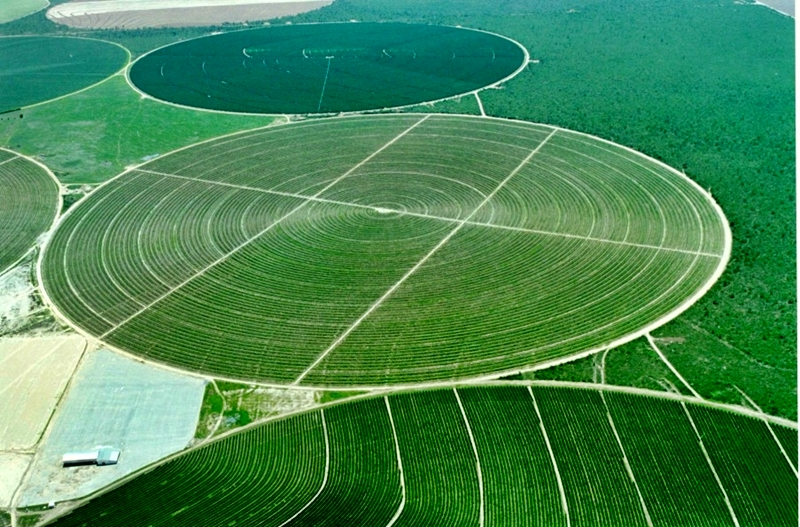
\includegraphics[width=0.76\textwidth]{figures/pivos_matopiba_cerrado.jpg}
  \caption{Irrigação com pivôs centrais no Cerrado do MATOPIBA, expressando a conversão intensiva das áreas de recarga em chapadões. Fonte: Acervo didático CHF662.}
  \label{fig:pivos_matopiba}
\end{figure}

Na quarta frente, associada ao \textbf{acesso desigual à água e à permanência territorial no Semiárido}, políticas historicamente centradas no ``combate à seca'' privilegiaram grandes açudes e obras concentradas em propriedades privadas, mantendo populações rurais dependentes de carros-pipa em estiagens. Em resposta a essa lógica concentradora, comunidades quilombolas (Figura~\ref{fig:quilombo_territorio}), associações rurais, movimentos sociais e universidades vêm consolidando estratégias de \textbf{convivência com o Semiárido}, articulando organização comunitária, tecnologias sociais descentralizadas de captação de água de chuva e manejo conservacionista do solo. O Exemplo 2.4 analisa a conectividade física e social entre chapadões convertidos e vales ocupados por comunidades tradicionais no Cerrado Baiano.

\begin{figure}[H]
  \centering
  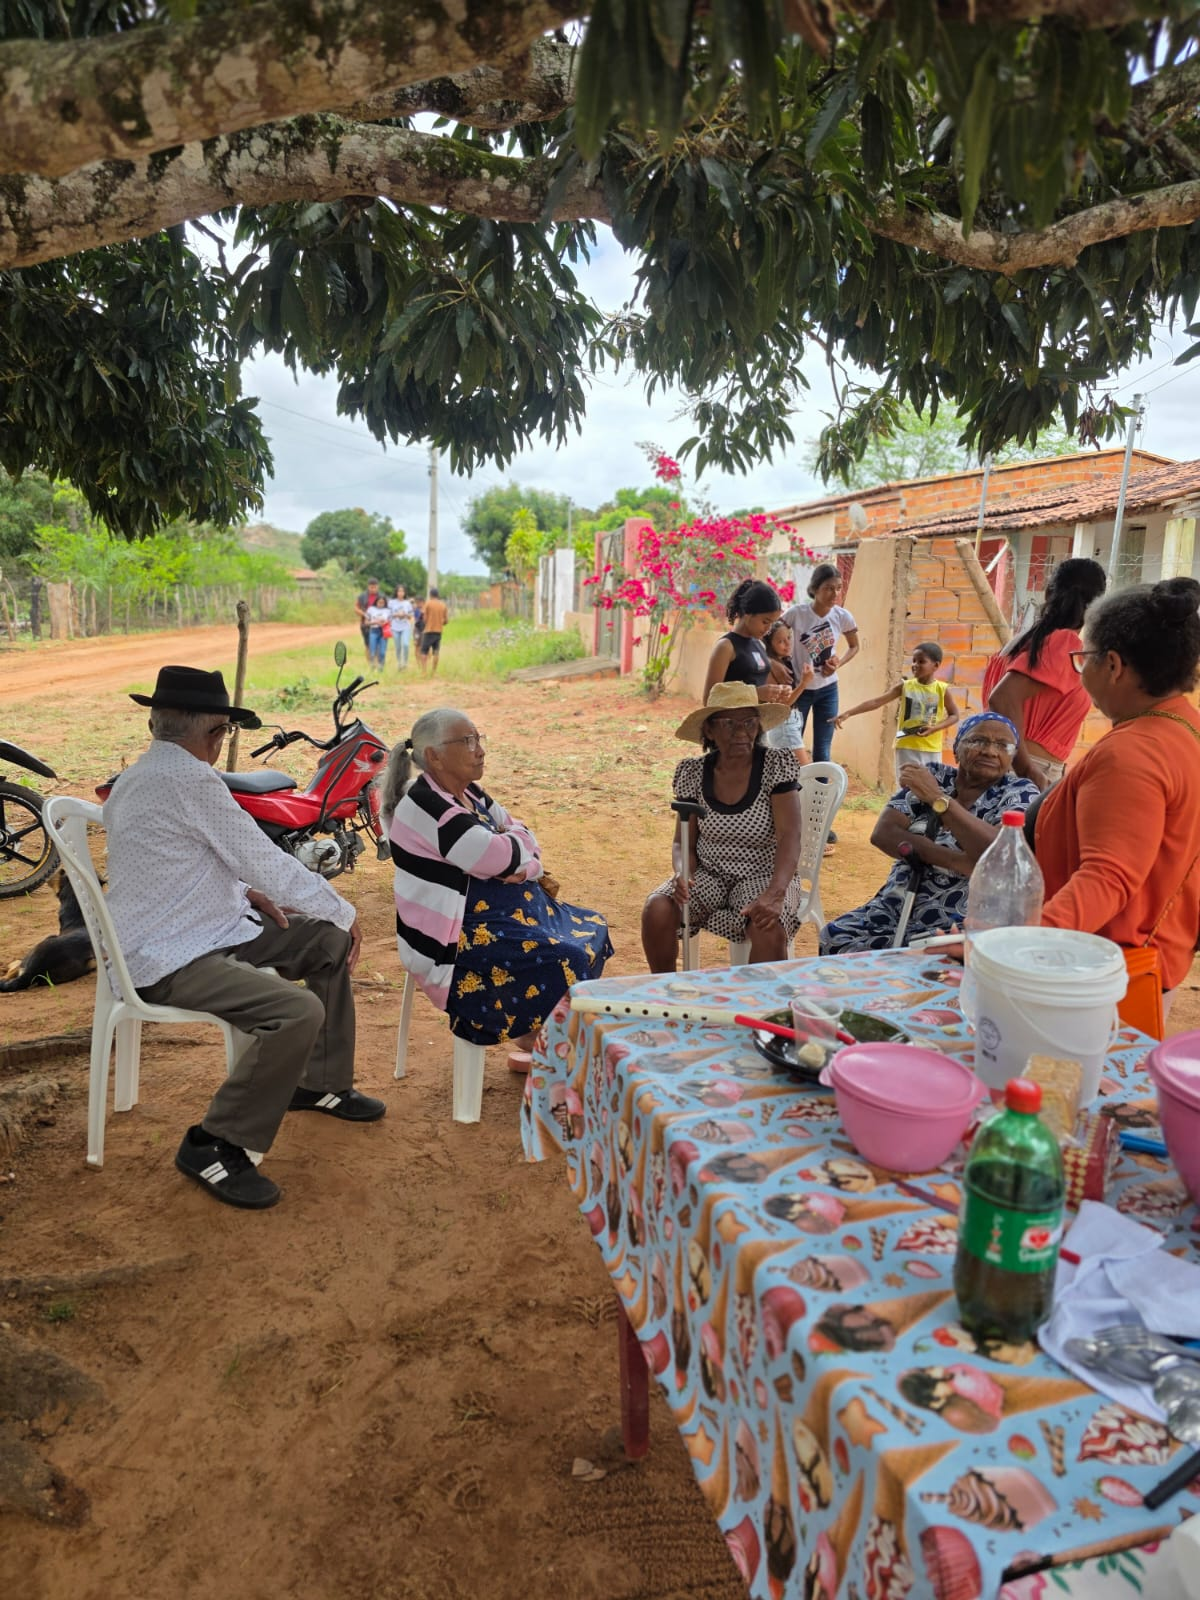
\includegraphics[width=0.76\textwidth]{figures/foto_quilombo_territorio.jpg}
  \caption{Comunidade quilombola de Tranqueira (BA), representando territorialidade tradicional, permanência comunitária e manejo adaptado ao ambiente semiárido. Fonte: Projeto Catuxe/UEFS.}
  \label{fig:quilombo_territorio}
\end{figure}

\begin{boxExemplo}{2.4 (Intermediário)}{Expansão da Fronteira Agrícola e Abordagem Socioambiental no Cerrado Baiano}
\passoEnunciado{Em uma sub-bacia fictícia de chapadão no Oeste Baiano \textit{(cenário didático ilustrativo)}, com área total de $40.000\text{ ha}$, o mapeamento de cobertura vegetal mostrou que, em 15 anos, a vegetação nativa de Cerrado reduziu-se de $32.000\text{ ha}$ para $14.000\text{ ha}$, substituída por lavouras mecanizadas irrigadas por pivôs centrais. Paralelamente, comunidades de fecho de pasto situadas nos vales a jusante relatam redução na vazão de veredas que utilizavam para cultivo de subsistência e criação extensiva.}
\passoDados{Área da sub-bacia de $40.000\text{ ha}$; Cerrado nativo reduzido de $32.000\text{ ha}$ para $14.000\text{ ha}$ em 15 anos; expansão de pivôs centrais no topo do chapadão; redução de vazão em veredas usadas por comunidades de fecho de pasto a jusante.}
\passoPedido{Calcular a área convertida e o percentual da sub-bacia que perdeu vegetação nativa nesse intervalo, construindo uma leitura integrada do caso segundo a Geografia Socioambiental de Mendonça (2001).}
\passoMetodo{Quantificação da conversão de cobertura vegetal seguida de análise dialética entre dinâmica físico-hidrológica (recarga no chapadão e descarga nas veredas) e conflito territorial (Mendonça, 2001).}
\passoContas{%
\textbf{Passo 1, Quantificação da perda de Cerrado.} A variação absoluta é $\Delta A = 14.000 - 32.000 = -18.000\text{ ha}$, correspondendo a $\frac{18.000}{40.000} \times 100\% = 45{,}0\%$ da sub-bacia e a $\frac{18.000}{32.000} \times 100\% = 56{,}25\%$ do Cerrado existente no início do período.\\
\textbf{Passo 2, Leitura físico-hidrológica integrada.} Os chapadões arenosos do Cerrado funcionam como áreas estratégicas de infiltração e recarga subterrânea que alimentam nascentes e veredas nos vales. A conversão de $45\%$ da sub-bacia associada à captação intensiva por pivôs centrais altera o balanço hídrico local e reduz a contribuição para os cursos d'água a jusante.\\
\textbf{Passo 3, Leitura socioambiental (Mendonça, 2001).} Enquanto uma leitura puramente física mediria apenas a vazão das veredas e uma abordagem puramente social descreveria apenas a disputa fundiária, a Geografia Socioambiental une ambos os planos ao evidenciar que a produção do espaço pelo agronegócio intensivo no topo da bacia transfere custos hídricos e vulnerabilidade social para as comunidades tradicionais nos fundos de vale.}
\passoResposta{Foram convertidos $18.000\text{ ha}$ ($45{,}0\%$ da sub-bacia e $56{,}25\%$ do Cerrado inicial). Sob a Geografia Socioambiental (Mendonça, 2001), o rebaixamento das veredas evidencia a inseparabilidade entre conectividade hidrológica chapadão-vale e apropriação desigual do território.}
\passoVerificacao{Os cálculos fecham ($32.000 - 18.000 = 14.000\text{ ha}$, restando $35\%$ da sub-bacia com Cerrado nativo), e a interpretação respeita a lógica de bacia hidrográfica ao conectar uso do solo em área de recarga com impactos socioespaciais a jusante.}
\end{boxExemplo}

Reconhecer o papel das comunidades tradicionais na conservação de veredas e áreas de uso comum previne o erro clássico de igualar toda presença humana à degradação ambiental.

\begin{boxErro}[Erro 2.3: Reproduzir o Mito da ``Natureza Intocada'' na Conservação Ambiental]
\textbf{Equívoco frequente:} supor que toda presença humana degrada o ambiente na mesma medida e que conservar significa necessariamente esvaziar territórios de seus habitantes tradicionais.

\textbf{Por que está incorreto:} como aponta Porto-Gonçalves (2006), essa postura reproduz a cisão cartesiana entre humano e natural, equiparando sistemas comunitários de baixo impacto a empreendimentos industriais de alta degradação.

\textbf{Como evitar:} analise empiricamente as práticas reais de uso da terra e reconheça que populações tradicionais frequentemente atuam como guardiãs da sociobiodiversidade.
\end{boxErro}

\section{Introdução à Abordagem Socioambiental na Geografia (Mendonça, 2001)}

Diante das limitações do dualismo cartesiano e da intensidade dos conflitos territoriais contemporâneos, a Geografia brasileira desenvolveu esforços consistentes para superar a separação entre o estudo da natureza e o estudo da sociedade. Um marco de referência desse movimento é o artigo \emph{Geografia socioambiental}, publicado por Francisco Mendonça na revista \emph{Terra Livre} (n. 16, 2001, p. 139--158). Mendonça (2001) questiona o uso genérico do termo ``ambiental'' quando reduzido exclusivamente à esfera natural (relevo, clima, fauna e flora) sem incorporar sujeitos históricos, desigualdade social e relações de poder. Por isso, o autor defende a adoção deliberada do prefixo \textbf{``socio-''} na expressão \textbf{Geografia Socioambiental}, afirmando desde a própria denominação que os problemas ambientais só podem ser compreendidos na interação dialética entre natureza e sociedade.

Essa introdução à abordagem socioambiental estabelece princípios metodológicos que serão aprofundados no Capítulo~3. A \textbf{superação da dicotomia físico-humana} articula as especificidades da geomorfologia, da climatologia e da geografia agrária diante de problemas concretos em que processos naturais e sociais se coproduzem. A \textbf{centralidade da sociedade na problemática ambiental} reconhece que enchentes urbanas, erosão acelerada, desertificação ou escassez hídrica atingem os grupos sociais de forma desigual conforme a vulnerabilidade e a organização do espaço. Além disso, o \textbf{compromisso com o diagnóstico e a intervenção territorial} combina rigor teórico-metodológico e relevância social para subsidiar políticas públicas, licenciamento, regras de alocação de água e recuperação de áreas degradadas. Esses quatro eixos, compreendendo a ruptura cartesiana na modernidade, a natureza como construção histórica (Porto-Gonçalves, 2006), os conflitos socioambientais na Bahia e no Nordeste e a abordagem socioambiental (Mendonça, 2001), formam a base direta para a elaboração do Estudo Orientado 1 (EO1) e conduzem à formalização do Sistema GTP no Capítulo~3.

% ----------------------------------------------------------------------------
% ETAPA 4 - SÍNTESE AVANÇADA E ESTUDO DE CASO INTEGRADOR
% ----------------------------------------------------------------------------
\etapa{4}{Síntese Avançada: Barragens, Temporalidades e Conflito Territorial}

Grandes obras de regularização fluvial oferecem um laboratório privilegiado para observar como a racionalidade instrumental, a imposição do tempo linear sobre os pulsos naturais e a desconsideração das territorialidades locais convergem no mesmo vale. O Exemplo 2.5 integra Porto-Gonçalves (2006) e Mendonça (2001) na avaliação socioambiental de uma barragem nordestina.

\begin{boxExemplo}{2.5 (Avançado)}{Barragem Fluvial, Descompasso de Temporalidades e Conflito Territorial}
\passoEnunciado{A construção de uma barragem de médio porte em um vale fluvial nordestino \textit{(cenário didático ilustrativo)} regularizou a vazão do rio para garantir geração elétrica e fornecimento constante a um perímetro agroindustrial. Cinco anos após o enchimento do reservatório, observam-se três efeitos encadeados, compreendendo a perda da prática secular de agricultura de vazante por comunidades ribeirinhas reassentadas em terrenos secos, a redução da deposição natural de nutrientes nas várzeas a jusante com intensificação da erosão marginal pela retenção de sedimentos no reservatório, e o declínio da pesca artesanal devido à barreira física à migração de peixes e à homogeneização do pulso de cheias.}
\passoDados{Obra de regularização fluvial voltada à geração elétrica e irrigação intensiva; três efeitos após 5 anos envolvendo perda da agricultura de vazante pós-reassentamento, retenção de sedimentos com erosão marginal a jusante e declínio da pesca artesanal.}
\passoPedido{Analisar o caso integrando a racionalidade instrumental e o descompasso entre tempo do capital e tempo ecológico, a concepção de natureza subjacente à obra (Porto-Gonçalves, 2006) e diretrizes de diagnóstico sob a ótica da Geografia Socioambiental (Mendonça, 2001).}
\passoMetodo{Síntese teórico-metodológica articulando Porto-Gonçalves (2006, p. 8--36), Mendonça (2001) e processos hidrossedimentológicos fluviais básicos.}
\passoContas{%
\textbf{Passo 1, Racionalidade instrumental e temporalidades.} O projeto tratou o rio sob o tempo linear e contínuo da produção industrial (vazão regularizada o ano inteiro), suprimindo o pulso sazonal de cheias e vazantes que estruturava tanto o ecossistema aquático (reprodução de peixes e renovação sedimentar das várzeas) quanto o calendário agrícola das famílias ribeirinhas.\\
\textbf{Passo 2, Concepção moderna de natureza (Porto-Gonçalves, 2006).} O rio foi concebido como tubulação hidráulica ou estoque de energia potencial a ser domado pela engenharia, ignorando que, para os ribeirinhos, ele constitui um território de vida historicamente construído. O reassentamento em terras secas pressupôs que qualquer lote substitui outro, apagando a especificidade ecológica e cultural da várzea.\\
\textbf{Passo 3, Diretrizes de diagnóstico socioambiental (Mendonça, 2001).} Um diagnóstico rigoroso deve avaliar a bacia inteira (montante, reservatório e jusante) com balanço de sedimentos e estabilidade de margens, mapear territorialidades tradicionais e dependência direta dos pulsos hidrológicos antes do licenciamento, e propor regras de vazões ambientais (hidrograma ecológico) acompanhadas de reparação territorial e participação comunitária na gestão do reservatório.}
\passoResposta{O caso evidencia como a racionalidade instrumental transforma um sistema fluvial vivo em infraestrutura setorial, rompendo simultaneamente processos hidrossedimentológicos e modos de vida ribeirinhos; a Geografia Socioambiental exige diagnosticar a bacia de forma integrada e reconhecer os sujeitos territoriais afetados.}
\passoVerificacao{A análise confirma a interdependência entre físico e social, pois a retenção de sedimentos pela barragem gera erosão marginal a jusante, empobrece várzeas e compromete a segurança alimentar e a renda das comunidades.}
\end{boxExemplo}

% ----------------------------------------------------------------------------
% ETAPA 5 - ARMADILHA CONCEITUAL E MATERIAIS AUDIOVISUAIS DE APOIO
% ----------------------------------------------------------------------------
\etapa{5}{Armadilha Conceitual e Materiais Audiovisuais de Apoio}

Ao aplicar a Geografia Socioambiental em trabalhos acadêmicos e relatórios técnicos, um erro frequente consiste em justapor capítulos independentes sobre o meio físico e a sociedade, mantendo intacta a cisão cartesiana sob nova nomenclatura.

\begin{boxErro}[Erro 2.4: Reduzir a Geografia Socioambiental à Justaposição de Física e Humana]
\textbf{Equívoco frequente:} acreditar que aplicar Mendonça (2001) consiste em escrever uma seção sobre clima e solo e outra seção independente sobre população e economia.

\textbf{Por que está incorreto:} justapor capítulos paralelos mantém intacta a dicotomia clássica da Geografia. A abordagem socioambiental exige mostrar como processos naturais e dinâmicas sociais interagem e se modificam reciprocamente no mesmo espaço.

\textbf{Como evitar:} formule suas análises a partir de nexos causais integrados, explicando como o modelo de ocupação de uma encosta ou bacia altera processos erosivos e concentra riscos sobre grupos vulneráveis.
\end{boxErro}

Para aprofundar os temas históricos e conceituais da relação sociedade-natureza na modernidade, assista às videoaulas indicadas na página da disciplina, iniciando por \textit{Relações de apropriação e transformação da natureza pelas sociedades humanas} (\url{https://www.youtube.com/watch?v=HX13IX_4290}) e complementando com \textit{Gestão Ambiental - Conceitos e Evolução das questões ambientais} (\url{https://www.youtube.com/watch?v=9eDzntrUvHY}), que contextualizam a trajetória histórica do pensamento ambiental e os modos de apropriação territorial.

% ----------------------------------------------------------------------------
% ETAPA 6 - EXERCÍCIOS DE FIXAÇÃO
% ----------------------------------------------------------------------------
\etapa{6}{EXERCÍCIOS DE FIXAÇÃO}

\subsection*{Nível 1: Básicos (Compreensão Conceitual)}

\begin{enumerate}[leftmargin=1.8em, itemsep=4pt]
  \item Explique em que consiste a \emph{ruptura cartesiana} entre sociedade e natureza na modernidade e aponte uma consequência direta dessa cisão para a organização da Geografia clássica.
  \espacoResolucao[1.8cm]

  \item Com base em Porto-Gonçalves (2006, p. 8--36), esclareça o significado da afirmação de que a natureza é uma \emph{construção social e histórica}, cuidando para preservar o reconhecimento da materialidade dos processos físicos.
  \espacoResolucao[1.8cm]

  \item Diferencie \emph{elemento natural} de \emph{recurso natural}, ilustrando com um exemplo concreto da realidade baiana ou nordestina.
  \espacoResolucao[1.8cm]

  \item Explique o descompasso entre o \emph{tempo do capital} e o \emph{tempo da natureza} no contexto da racionalidade instrumental moderna.
  \espacoResolucao[1.8cm]

  \item Segundo Francisco Mendonça (2001), qual é a justificativa teórica e metodológica para o uso do prefixo ``socio-'' na expressão \emph{Geografia Socioambiental}?
  \espacoResolucao[1.8cm]

\subsection*{Nível 2: Intermediários (Análise Crítica e Aplicação)}

  \item Analise o paradoxo apontado por Porto-Gonçalves (2006) entre a exploração predatória da natureza como mercadoria e a defesa de uma ``natureza intocada'' sem presença humana. O que essas duas visões têm em comum?
  \espacoResolucao[1.8cm]

  \item Escolha uma das quatro frentes de conflito socioambiental discutidas no capítulo (expansão energética no Semiárido, barragens fluviais, fronteira agrícola no Oeste Baiano ou acesso desigual à água) e identifique o recurso apropriado, os principais atores em disputa e dois impactos físico-bióticos articulados a efeitos sociais.
  \espacoResolucao[1.8cm]

  \item Em um cenário didático ilustrativo, um reservatório comunitário no Semiárido dispõe de $90.000\text{ m}^3$ de volume útil para 200 dias de estiagem. Duas demandas disputam essa água, sendo 150 famílias que consomem $0{,}6\text{ m}^3/\text{dia}$ cada e um empreendimento externo que solicita autorização para captar $400\text{ m}^3/\text{dia}$. Calcule a demanda total de cada parte no período, verifique se há déficit e analise o caso sob a ótica dos conflitos socioambientais.
  \espacoResolucao[1.8cm]

  \item Diferencie as políticas históricas de ``combate à seca'' das estratégias contemporâneas de ``convivência com o Semiárido'', relacionando essa distinção à racionalidade instrumental e à justiça socioambiental.
  \espacoResolucao[1.8cm]

  \item Elabore um parágrafo analítico demonstrando como a abordagem socioambiental (Mendonça, 2001) supera tanto o naturalismo redutor quanto o sociologismo que ignora o suporte físico-biótico do território.
  \espacoResolucao[1.8cm]

\subsection*{Nível 3: Aplicados e Objetivos (Múltipla Escolha)}

  \item Na análise de Porto-Gonçalves (2006, p. 8--36) sobre a formação histórica da questão ambiental na modernidade, a separação entre sociedade e natureza:
  \begin{alternativas}
    \item É uma característica biológica universal presente de forma idêntica em todas as culturas humanas desde a pré-história.
    \item Consolida-se historicamente com o pensamento moderno-cartesiano, instituindo a natureza como objeto externo e passivo a ser dominado pela ciência e pela técnica.
    \item Foi completamente superada pela Revolução Industrial, que reintegrou o ritmo produtivo das fábricas aos ciclos lentos dos ecossistemas.
    \item Refere-se exclusivamente à divisão administrativa entre zonas urbanas e zonas rurais nos municípios brasileiros.
    \item Impediu o desenvolvimento das ciências da natureza, pois o mecanicismo cartesiano rejeitava qualquer estudo matemático do mundo físico.
  \end{alternativas}
  \espacoResolucao[1.8cm]

  \item Sobre o processo pelo qual um elemento biofísico passa a ser tratado como \emph{recurso natural}, é \textbf{correto} afirmar que:
  \begin{alternativas}
    \item Todo elemento físico da crosta terrestre é automaticamente um recurso econômico, independentemente da técnica ou da organização social existente.
    \item A transformação de elementos da natureza em recursos naturais depende de condições técnicas, econômicas, culturais e políticas historicamente situadas.
    \item Recursos renováveis, como o vento e a energia solar, jamais geram impactos ambientais ou conflitos territoriais quando apropriados em larga escala.
    \item A apropriação de recursos naturais sob racionalidade instrumental respeita integralmente o tempo geológico de formação dos solos e de recarga dos aquíferos.
    \item A noção de recurso natural é neutra e alheia às disputas fundiárias ou à produção do espaço geográfico.
  \end{alternativas}
  \espacoResolucao[1.8cm]

  \item No contexto da Bahia e do Nordeste, a expansão de parques eólicos em áreas serranas da Caatinga exemplifica um conflito socioambiental porque:
  \begin{alternativas}
    \item A geração eólica produz grandes volumes de gases de efeito estufa diretamente na atmosfera do Semiárido durante a rotação das pás.
    \item Embora utilize fonte renovável, a apropriação espacial das serras provoca supressão vegetal, erosão na base das torres, interferência na avifauna e tensões fundiárias com comunidades locais.
    \item Os ventos do Semiárido são insuficientes para movimentar turbinas, tornando a região tecnicamente inviável para energia eólica.
    \item As comunidades locais opõem-se por princípio a qualquer forma de energia elétrica, recusando-se a utilizar eletricidade em suas residências.
    \item Os impactos físicos das obras restringem-se ao interior das subestações urbanas, sem atingir o relevo, os solos ou a vegetação da Caatinga.
  \end{alternativas}
  \espacoResolucao[1.8cm]

  \item De acordo com a proposta de \emph{Geografia Socioambiental} formulada por Francisco Mendonça (2001):
  \begin{alternativas}
    \item O estudo ambiental deve restringir-se aos fenômenos climáticos e geomorfológicos naturais, evitando interferência de temas sociais e políticos.
    \item A Geografia Física deve ser extinta dos cursos de graduação, pois apenas a análise econômica explica a degradação do espaço.
    \item A incorporação do termo ``socioambiental'' busca superar a dicotomia físico-humana, compreendendo o ambiente a partir da interação indissociável entre natureza e sociedade.
    \item Os desastres e a degradação ambiental atingem de maneira uniforme todas as classes sociais, independentemente da organização do território.
    \item A abordagem socioambiental consiste em anexar um capítulo de demografia ao final de relatórios geomorfológicos sem estabelecer relações causais entre eles.
  \end{alternativas}
  \espacoResolucao[1.8cm]

  \item Em um cenário didático ilustrativo, uma comunidade tradicional de fundo de pasto e uma empresa agroindustrial disputam o uso das águas de um riacho que nasce em área de chapadão. A análise desse episódio como \textbf{conflito socioambiental} exige reconhecer que:
  \begin{alternativas}
    \item Trata-se apenas de um mal-entendido de comunicação que desaparece assim que a empresa apresentar seu catálogo comercial.
    \item Existe confronto entre diferentes racionalidades, interesses e modos de apropriação do território e da água, com efeitos diretos sobre a dinâmica hidrológica e a reprodução social.
    \item O conflito só tem relevância geográfica se houver alteração na precipitação média anual registrada na estação meteorológica mais próxima.
    \item A solução técnica adequada consiste em transferir integralmente o controle da bacia ao agente de maior capacidade de investimento financeiro.
    \item A análise deve desconsiderar o uso do solo na área de recarga do chapadão, pois a questão pertence exclusivamente ao direito privado.
  \end{alternativas}
  \espacoResolucao[1.8cm]
\end{enumerate}

% ----------------------------------------------------------------------------
% ETAPA 7 - QUESTÕES DE PROVAS, ENADE E CONCURSOS AMBIENTAIS
% ----------------------------------------------------------------------------
\etapa{7}{QUESTÕES DE PROVAS, ENADE E CONCURSOS AMBIENTAIS}

\begin{enumerate}[leftmargin=1.8em, itemsep=5pt, start=16]
  \item \textbf{(Questão autoral, estilo ENADE / Concurso Ambiental)} Leia o excerto adaptado dos debates epistemológicos da Geografia contemporânea: \emph{``Toda sociedade, toda cultura cria, inventa, institui uma determinada ideia do que seja a natureza. Nesse sentido, o conceito de natureza é criado e instituído historicamente pelos seres humanos.''} (em diálogo com Porto-Gonçalves, 2006). Com base nessa perspectiva e na formação histórica da questão ambiental na modernidade, assinale a alternativa \textbf{correta}:
  \begin{alternativas}
    \item A afirmação nega a existência física de processos geomorfológicos e hidrológicos, reduzindo o meio ambiente a uma ficção linguística sem base material.
    \item A ideia moderna de natureza como objeto externo e dominável serviu de suporte ideológico à apropriação instrumental dos territórios e ao aprofundamento da crise ambiental.
    \item A concepção cartesiana promoveu a reunificação harmoniosa entre cultura, religião, ecossistemas locais e economia industrial desde o século XVII.
    \item O conceito de natureza permaneceu imutável desde a Antiguidade até o século XXI, alterando-se apenas a tecnologia empregada na agricultura.
    \item A defesa de áreas naturais completamente isoladas da ação humana rompe definitivamente com a dicotomia moderna entre sociedade e natureza.
  \end{alternativas}
  \espacoResolucao[1.8cm]

  \item \textbf{(Questão autoral, estilo ENADE / Concurso Ambiental)} Considere a implantação de grandes barragens e a expansão da fronteira agrícola mecanizada em bacias hidrográficas do Nordeste brasileiro. Sob a perspectiva da produção do espaço geográfico e da Geografia Socioambiental (Mendonça, 2001), analise as proposições abaixo:
  \begin{enumerate}[label=\Roman*., leftmargin=1.6em, itemsep=1.5pt]
    \item A regularização artificial de vazões por barragens pode alterar a dinâmica hidrossedimentológica a jusante e desestruturar modos de vida ribeirinhos baseados no pulso natural de cheias e vazantes.
    \item A conversão acelerada de vegetação nativa em áreas de recarga hídrica conecta processos físico-hidrológicos a conflitos territoriais com comunidades situadas nos vales a jusante.
    \item O descompasso entre o tempo acelerado de retorno do capital e o tempo lento de regeneração edáfica e hidrológica intensifica quadros de degradação e vulnerabilidade socioambiental.
    \item Por envolverem obras de infraestrutura autorizadas pelo Estado, grandes empreendimentos hídricos e agrícolas são tecnicamente neutros e não constituem conflitos socioambientais.
  \end{enumerate}
  Estão corretas apenas as proposições:
  \begin{alternativas}
    \item I e IV.
    \item II e IV.
    \item I, II e III.
    \item II, III e IV.
    \item I, III e IV.
  \end{alternativas}
  \espacoResolucao[1.8cm]

  \item \textbf{(Questão autoral, estilo ENADE / Concurso Ambiental)} Em um concurso para Geógrafo(a) de órgão ambiental estadual, solicitou-se a escolha da diretriz metodológica mais coerente com a abordagem socioambiental (Mendonça, 2001) para diagnosticar conflitos de uso da terra e escassez hídrica em uma bacia do Semiárido Baiano. A alternativa que atende rigorosamente a essa diretriz é:
  \begin{alternativas}
    \item Elaborar exclusivamente o mapeamento geomorfológico e climático da bacia, deixando as questões de acesso à água e posse da terra fora do escopo do relatório técnico.
    \item Adotar o enfoque de ``combate à seca'' baseado unicamente em obras hidráulicas concentradas, dispensando o diagnóstico da cobertura vegetal e das práticas comunitárias.
    \item Integrar o levantamento dos processos físico-bióticos (relevo, solos, vegetação e dinâmica hídrica) à análise das relações sociais, dos conflitos de uso dos recursos e das vulnerabilidades territoriais.
    \item Substituir o levantamento de campo e os indicadores físicos por entrevistas de opinião, pois a abordagem socioambiental considera dispensáveis os dados da Geografia Física.
    \item Aplicar o mesmo modelo produtivo mecanizado em toda a bacia para padronizar o uso do solo e eliminar diferenças culturais entre os moradores.
  \end{alternativas}
  \espacoResolucao[1.8cm]
\end{enumerate}

\begin{boxDica}[Orientações para o Estudo Orientado 1 (EO1) e a Prova Dissertativa]
O \textbf{EO1} (valor $0{,}5$ ponto, entregue na Semana 2) exige leitura atenta de \textbf{Porto-Gonçalves (2006, p. 8--36)} e introdução a \textbf{Mendonça (2001)}. Para produzir uma resposta sólida no EO1 e na Prova Teórica (Semana 10):
\begin{enumerate}[leftmargin=1.5em, itemsep=2pt]
  \item \textbf{Evite resumos descritivos soltos,} articulando explicitamente a cadeia que vai da modernidade e ruptura cartesiana até a conversão da natureza em mercadoria, os conflitos socioambientais e a resposta da Geografia Socioambiental.
  \item \textbf{Dê concretude geográfica,} exemplificando conflitos socioambientais com processos reais da Bahia e do Nordeste (eólicas no Semiárido, barragens, Oeste Baiano ou acesso à água), sem inventar dados estatísticos.
  \item \textbf{Use vocabulário preciso,} distinguindo \emph{elemento natural} de \emph{recurso natural}, diferenciando \emph{construção social da ideia de natureza} de negação da materialidade física e justificando o papel do prefixo ``socio-'' em Mendonça (2001).
\end{enumerate}
\end{boxDica}

% ----------------------------------------------------------------------------
% ETAPA 8 - GABARITO COMENTADO (PÁGINA SEPARADA)
% ----------------------------------------------------------------------------
\clearpage
\etapa{8}{GABARITO COMENTADO}

\begin{boxGabarito}[Resolução Comentada: Nível 1 (Questões 1 a 5)]
\begin{enumerate}[leftmargin=1.8em, itemsep=4pt]
  \item \textbf{Ruptura cartesiana e Geografia clássica.} A ruptura cartesiana separou o sujeito racional humano (\emph{res cogitans}, sociedade e cultura) da matéria externa (\emph{res extensa}, natureza), concebendo a natureza como máquina passiva a ser dominada pela ciência e pela técnica. Na Geografia institucionalizada no século XIX, essa cisão manifestou-se na dicotomia entre uma Geografia Física voltada às leis naturais e uma Geografia Humana voltada à sociedade, muitas vezes desconectadas entre si.

  \item \textbf{Natureza como construção social e histórica (Porto-Gonçalves, 2006).} Afirmar que a natureza é socialmente construída pressupõe o reconhecimento da existência material de rios, rochas e processos físicos, destacando que o modo como cada sociedade define, significa, valoriza e se relaciona com o mundo natural varia histórica e culturalmente, do pertencimento comunitário em povos tradicionais à mercantilização na modernidade capitalista.

  \item \textbf{Elemento natural e recurso natural.} Um \emph{elemento natural} existe pela dinâmica biofísica da Terra independentemente de sua exploração econômica (como o regime de ventos nas serras da Caatinga ou as águas subterrâneas do Cerrado). Ele se torna \emph{recurso natural} quando um conjunto técnico, econômico e político o apropria e o valoriza para fins produtivos (como na instalação de parques eólicos com linhas de transmissão ou na perfuração de poços para irrigação mecanizada).

  \item \textbf{Tempo do capital e tempo da natureza.} Sob a racionalidade instrumental, o tempo econômico exige retorno rápido, intensificação contínua e expansão de fronteiras em poucos anos, ao passo que os processos ecológicos e pedogenéticos (formação do solo, regeneração da Caatinga, recarga de aquíferos) operam em escalas lentas de décadas ou séculos. Esse descompasso produz exaustão de solos, sobre-exploração hídrica e perda de resiliência ambiental.

  \item \textbf{O prefixo ``socio-'' em Mendonça (2001).} Mendonça (2001) adota ``Geografia Socioambiental'' para enfatizar que a problemática ambiental abrange indissociavelmente os elementos físico-bióticos, a sociedade, seus conflitos, suas desigualdades e o modo como o espaço é produzido e apropriado.
\end{enumerate}
\end{boxGabarito}

\begin{boxGabarito}[Resolução Comentada: Nível 2 (Questões 6 a 10)]
\begin{enumerate}[leftmargin=1.8em, itemsep=4pt, start=6]
  \item \textbf{Paradoxo da exploração predatória e da ``natureza intocada'' (Porto-Gonçalves, 2006).} Embora pareçam opostas, ambas as visões compartilham o mesmo fundamento cartesiano ao separar rigidamente seres humanos e natureza. Enquanto o produtivismo exclui a natureza da esfera ética para explorá-la como mercadoria, o preservacionismo excludente exclui populações tradicionais da natureza ao presumir que qualquer presença humana é igualmente destrutiva.

  \item \textbf{Análise de uma frente socioambiental (resposta-modelo para expansão eólica no Semiárido).} O recurso apropriado compreende o regime de ventos e as áreas serranas da Caatinga; os atores em disputa reúnem empresas geradoras de energia, proprietários de terra, Estado e comunidades rurais ou de fundo de pasto; e os impactos físico-bióticos articulados a efeitos sociais incluem abertura de acessos com compactação e erosão na base das torres (degradando pastagens nativas usadas pelas famílias), além do cercamento de áreas comuns e ruído contínuo que alteram o uso comunitário e a qualidade de vida local. Qualquer uma das outras três frentes analisadas na Etapa 3 é igualmente válida se apresentar recurso, atores e impactos físico-sociais com rigor.

  \item \textbf{Cálculo e análise do cenário didático ($90.000\text{ m}^3$).}
  A demanda comunitária das 150 famílias corresponde a $Q_{\text{fam}} = 150 \times 0{,}6 = 90\text{ m}^3/\text{dia}$, totalizando $V_{\text{fam}} = 90 \times 200 = 18.000\text{ m}^3$ ($20\%$ do reservatório). A demanda do empreendimento externo soma $V_{\text{emp}} = 400 \times 200 = 80.000\text{ m}^3$ ($88{,}9\%$ do reservatório). Somadas, as demandas atingem $V_{\text{total}} = 18.000 + 80.000 = 98.000\text{ m}^3$, gerando saldo de $90.000 - 98.000 = -8.000\text{ m}^3$ (déficit de $8.000\text{ m}^3$, mesmo desconsiderando a evaporação). Como o reservatório supriria cinco vezes a necessidade básica das 150 famílias, o déficit decorre da concentração de $81{,}6\%$ da demanda total ($\frac{80.000}{98.000}$) em um único agente externo, configurando conflito socioambiental distributivo pelo acesso à água.

  \item \textbf{``Combate à seca'' e ``convivência com o Semiárido''.} O ``combate à seca'' apoia-se na racionalidade instrumental que tenta vencer o clima com grandes obras centralizadas, historicamente associadas à concentração fundiária e hídrica. A ``convivência com o Semiárido'' reconhece as características ecológicas da Caatinga e do regime pluviométrico, promovendo tecnologias sociais descentralizadas de captação, conservação do solo e democratização do acesso à água com justiça socioambiental.

  \item \textbf{Superação do naturalismo e do sociologismo (Mendonça, 2001).} A Geografia Socioambiental recusa tanto o naturalismo que analisa relevo, clima e hidrografia isolados da sociedade, da economia e do conflito, quanto o sociologismo que discute disputas sociais abstraídas da materialidade do solo, da água e dos ecossistemas. Ao integrar os dois polos em nexos causais concretos, explica simultaneamente a dinâmica física da degradação e a distribuição social das vulnerabilidades.
\end{enumerate}
\end{boxGabarito}

\begin{boxGabarito}[Resolução Comentada: Nível 3 e Questões de Provas/Concursos (Questões 11 a 18)]
\begin{enumerate}[leftmargin=1.8em, itemsep=4pt, start=11]
  \item \textbf{Gabarito: (B).} Porto-Gonçalves (2006) mostra que a separação sujeito-objeto consolidada na modernidade cartesiana instituiu a natureza como matéria externa e passiva a ser controlada pela técnica. As alternativas (A), (C), (D) e (E) erram ao universalizar a visão moderna para toda a história, afirmar que a Revolução Industrial reintegrou ciclos ecológicos, reduzir o processo a limites administrativos ou negar a matematização cartesiana da física.

  \item \textbf{Gabarito: (B).} Um elemento natural passa à condição de recurso natural quando incorporado por técnicas, demandas econômicas e arranjos políticos historicamente situados. As demais alternativas desconsideram a historicidade técnica e social do conceito, supõem neutralidade em fontes renováveis de grande escala ou afirmam respeito automático aos tempos geológicos.

  \item \textbf{Gabarito: (B).} A geração eólica utiliza fonte renovável, mas sua implantação espacial na Caatinga envolve supressão vegetal, erosão na base das torres, interferência na avifauna e conflitos fundiários e contratuais com comunidades locais, ocorrendo justamente nas serras e áreas rurais de implantação.

  \item \textbf{Gabarito: (C).} Mendonça (2001) propõe a Geografia Socioambiental exatamente para superar a dicotomia físico-humana e analisar o ambiente como interação indissociável entre natureza e sociedade, evitando reducionismos unilaterais e justaposições sem nexos causais.

  \item \textbf{Gabarito: (B).} Um conflito socioambiental envolve disputa entre diferentes projetos, racionalidades e modos de uso do território e dos recursos hídricos, com impactos materiais sobre a bacia e a reprodução social, inclusive quando a precipitação média permanece constante.

  \item \textbf{Gabarito: (B).} A instituição moderna da natureza como objeto externo e passivo legitimou sua apropriação instrumental e a intensificação da degradação ambiental (Porto-Gonçalves, 2006), sem negar a materialidade física dos processos geomorfológicos e hidrológicos.

  \item \textbf{Gabarito: (C).} As proposições I, II e III articulam corretamente a dinâmica física (sedimentos, recarga hídrica, tempo ecológico) e os conflitos territoriais (ribeirinhos, comunidades de vale, vulnerabilidade socioambiental). A proposição IV é falsa porque autorização estatal ou grande porte técnico mantém possibilidades concretas de conflito socioambiental.

  \item \textbf{Gabarito: (C).} A diretriz coerente com Mendonça (2001) integra os processos físico-bióticos (relevo, solos, vegetação, água) à análise das relações sociais, conflitos de uso e vulnerabilidades territoriais, preservando dados físicos de campo em diálogo com a realidade social.
\end{enumerate}
\end{boxGabarito}

% ----------------------------------------------------------------------------
% ETAPA 9 - RESUMO DO CAPÍTULO
% ----------------------------------------------------------------------------
\begin{boxResumo}
\begin{itemize}[leftmargin=1.5em, itemsep=3pt]
  \item \textbf{Modernidade e ruptura cartesiana,} a ciência mecanicista moderna separou sujeito (sociedade) e objeto (natureza), legitimando a dominação técnica do mundo natural e influenciando a dicotomia histórica entre Geografia Física e Geografia Humana.
  \item \textbf{Natureza como construção social (Porto-Gonçalves, 2006, p. 8--36),} preservando a materialidade física dos processos naturais, cada sociedade institui historicamente o que entende por natureza, explicando o paradoxo entre exploração mercantil e mito da ``natureza intocada''.
  \item \textbf{Apropriação instrumental,} elementos biofísicos tornam-se ``recursos naturais'' e mercadorias sob técnicas e relações de poder específicas, opondo o tempo rápido do capital ao tempo lento dos ciclos ecológicos e pedogenéticos.
  \item \textbf{Conflitos socioambientais na Bahia e no Nordeste,} disputas pela produção do espaço manifestam-se em frentes como expansão eólica no Semiárido, barragens fluviais, fronteira agrícola no Oeste Baiano e acesso desigual à água (``combate à seca'' frente à ``convivência com o Semiárido'').
  \item \textbf{Geografia Socioambiental (Mendonça, 2001),} supera o naturalismo e o sociologismo isolados ao analisar o ambiente como interação dialética entre dinâmicas físico-bióticas, organização espacial e justiça socioambiental.
\end{itemize}
\end{boxResumo}

% ----------------------------------------------------------------------------
% ETAPA 10 - TESTE DE APRENDIZAGEM (CHECKPOINT)
% ----------------------------------------------------------------------------
\begin{boxTeste}
Responda sem consultar o capítulo e avalie sua preparação para o \textbf{Estudo Orientado 1 (EO1)}. Julgue cada item como Verdadeiro (\textbf{V}) ou Falso (\textbf{F}).
\begin{enumerate}[leftmargin=1.8em, itemsep=3pt]
  \item (\quad) A ruptura cartesiana contribuiu para que a natureza fosse concebida na modernidade como objeto externo, mensurável e passivo diante da dominação técnica.
  \item (\quad) Segundo Porto-Gonçalves (2006), defender que a natureza é uma construção social significa negar que processos físicos como erosão e chuvas tenham existência material objetiva.
  \item (\quad) A implantação de parques eólicos no Semiárido Baiano, embora baseada em fonte renovável, pode gerar impactos físico-bióticos e conflitos socioambientais em torno do uso da terra e da Caatinga.
  \item (\quad) A Geografia Socioambiental proposta por Mendonça (2001) busca integrar a dinâmica físico-natural e a organização socioespacial, superando a dicotomia clássica entre Geografia Física e Geografia Humana.
\end{enumerate}

\vspace{4pt}
\textbf{Gabarito do Checkpoint:} 1.~\V \quad|\quad 2.~\F \quad|\quad 3.~\V \quad|\quad 4.~\V

\textbf{Critério de domínio:} Acertou $\mathbf{\ge 3/4}$? Você domina a base conceitual necessária para entregar o \textbf{EO1} com rigor e avançar ao Capítulo 3 (EO2). Acertou $\mathbf{< 3/4}$? Revise especialmente os Erros 2.1 e 2.4 e as quatro frentes de conflito da Etapa 3 antes de redigir seu Estudo Orientado.
\end{boxTeste}
